\section{Testing Results}

\subsection{Environment and Timing Methodology}

\begin{table}[H]
\centering
\small
\caption{Measured experiment environment.}
\begin{tabularx}{\textwidth}{lX}
\toprule
Item & Configuration \\
\midrule
Experiment date & 2026-10-03 \\
CPU & AMD Ryzen 7 H 255 W/ Radeon 780M \\
Operating system & WSL2; Linux 6.6.87.2-microsoft-standard-WSL2; x86-64 \\
Compiler & gcc (Ubuntu 13.3.0-6ubuntu2\textasciitilde{}24.04.1) 13.3.0 \\
Build flags & -std=c11 -O2 -Wall -Wextra -Wpedantic \\
Timer & POSIX CLOCK\_MONOTONIC, elapsed wall time \\
Repetitions & 3 for each scenario / size / tree \\
Execution & One process; sequential; no CPU affinity \\
B+ capacity & 32 leaf records or 32 internal children \\
\bottomrule
\end{tabularx}
\end{table}
\FloatBarrier

Insertion and deletion are timed separately with CLOCK\_\allowbreak{}MONOTONIC. Allocation and freeing inside tree operations are included; input generation, file output, and membership checks are excluded. A 256-key untimed run warms each implementation, and the execution order rotates across trials. Between the timed phases, 256 read-only queries sample inserted keys; after deletion, the driver requires a NULL root. No structural invariant checker runs in the current driver. The queries may warm deletion caches.

\subsection{Smoke Test}

\begin{table}[H]
\centering
\small
\caption{Observed smoke test results.}
\begin{tabularx}{\textwidth}{XlX}
\toprule
Test case & Type & Expected / actual result \\
\midrule
Deleting from an empty tree & Boundary & Accepted, no change; PASS for all five trees \\
INT\_MIN and INT\_MAX; 1,000 increasing keys & Functional & Both boundary keys found; sampled keys found; an absent key reported absent \\
Full insert-then-delete cycle & Functional & Every key accepted, then removed; NULL root afterwards; PASS \\
Same cycle under ASan and UBSan & Memory / undefined behavior & No sanitizer diagnostics; PASS \\
All 315 timed trials, N up to 100,000 & Large-scale & Sampled keys present after insertion; NULL root after deletion; PASS \\
\bottomrule
\end{tabularx}
\end{table}
\FloatBarrier

README.md documents how to reproduce every result in this chapter: make check runs the cycle above, make sanitize repeats it under AddressSanitizer and UndefinedBehaviorSanitizer, and make benchmark regenerates all input files and timings. The checks.log file retains the compiler commands and the PASS output from both builds. Sanitizers detect exercised memory errors and undefined behavior, but do not verify AVL height balance, red-black black heights, or B+ occupancy and separator invariants. The smoke test checks sampled membership and a full deletion cycle; it does not replace those structural checks.

\subsection{Runtime Tables}

All values below are milliseconds. Each total is the median of three per-trial insertion-plus-deletion sums. The separate insertion and deletion medians are computed independently and need not add exactly to the median total. Minimum and maximum values describe the three observed runs, not confidence intervals. Exact second-valued measurements are retained in raw.csv.

\Needspace{12\baselineskip}
\subsubsection{Increasing insertion / increasing deletion}

\begin{table}[H]
\centering
\small
\caption{Increasing insertion / increasing deletion: median total elapsed time (ms).}
\begin{tabular}{lrrrrr}
\toprule
N & BST & AVL & Splay & RedBlack & BPlus32 \\
\midrule
1,000 & 1.151 & 0.055 & 0.027 & 0.143 & 0.054 \\
2,000 & 4.646 & 0.202 & 0.084 & 0.392 & 0.186 \\
5,000 & 27.751 & 0.408 & 0.176 & 0.876 & 0.394 \\
10,000 & 111.839 & 1.163 & 0.447 & 2.279 & 1.012 \\
20,000 & 444.720 & 1.644 & 0.788 & 4.374 & 1.797 \\
50,000 & 2757.504 & 7.110 & 1.843 & 14.321 & 5.003 \\
100,000 & 10999.209 & 16.004 & 3.402 & 37.267 & 11.107 \\
\bottomrule
\end{tabular}
\end{table}
\FloatBarrier

\Needspace{12\baselineskip}
\subsubsection{Increasing insertion / reverse deletion}

\begin{table}[H]
\centering
\small
\caption{Increasing insertion / reverse deletion: median total elapsed time (ms).}
\begin{tabular}{lrrrrr}
\toprule
N & BST & AVL & Splay & RedBlack & BPlus32 \\
\midrule
1,000 & 2.348 & 0.087 & 0.036 & 0.179 & 0.100 \\
2,000 & 9.652 & 0.173 & 0.097 & 0.321 & 0.209 \\
5,000 & 57.488 & 0.422 & 0.195 & 0.839 & 0.592 \\
10,000 & 219.320 & 0.708 & 0.381 & 1.763 & 0.986 \\
20,000 & 886.977 & 1.621 & 0.779 & 4.072 & 2.177 \\
50,000 & 5483.877 & 5.159 & 1.950 & 13.683 & 6.083 \\
100,000 & 21933.532 & 15.375 & 3.894 & 36.391 & 14.964 \\
\bottomrule
\end{tabular}
\end{table}
\FloatBarrier

\Needspace{12\baselineskip}
\subsubsection{Random insertion / random deletion}

\begin{table}[H]
\centering
\small
\caption{Random insertion / random deletion: median total elapsed time (ms).}
\begin{tabular}{lrrrrr}
\toprule
N & BST & AVL & Splay & RedBlack & BPlus32 \\
\midrule
1,000 & 0.077 & 0.126 & 0.118 & 0.201 & 0.121 \\
2,000 & 0.172 & 0.298 & 0.296 & 0.430 & 0.241 \\
5,000 & 0.555 & 0.881 & 0.877 & 1.233 & 0.777 \\
10,000 & 1.283 & 2.471 & 2.521 & 3.278 & 2.421 \\
20,000 & 2.661 & 4.235 & 4.836 & 6.370 & 3.356 \\
50,000 & 9.664 & 15.876 & 15.423 & 19.003 & 10.389 \\
100,000 & 22.791 & 37.573 & 41.841 & 52.854 & 22.443 \\
\bottomrule
\end{tabular}
\end{table}
\FloatBarrier

\subsection{Runtime Plots}

The plots show insertion, deletion, and total elapsed time separately. Both axes are logarithmic so millisecond and multi-second results remain visible together. Corresponding phases use identical axis limits across scenarios. Distinct markers supplement colors. Points show medians; whiskers show observed minima and maxima. A line connecting tested sizes illustrates growth without asserting measurements at intermediate sizes.

\begin{figure}[htbp]
\centering
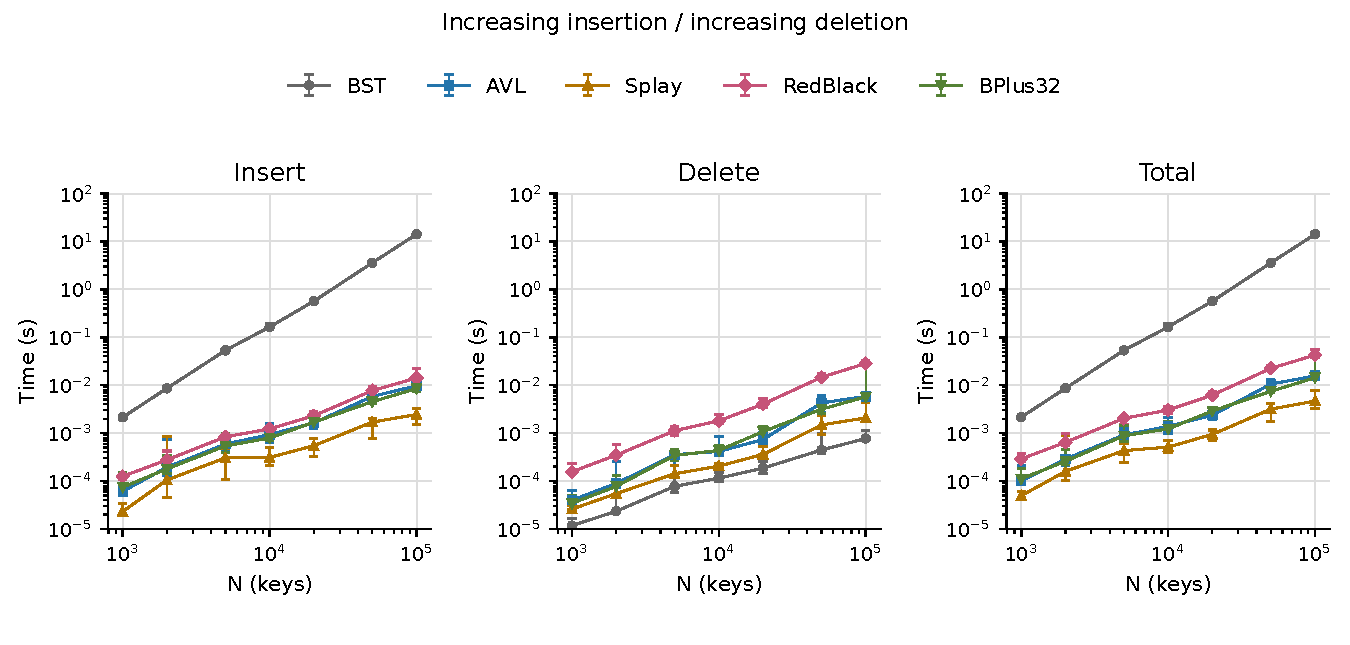
\includegraphics[width=\textwidth]{figures/increasing_same.pdf}
\caption{Increasing insertion / increasing deletion. Each phase uses the same scale as its counterpart in the other scenarios.}
\end{figure}

\begin{figure}[htbp]
\centering
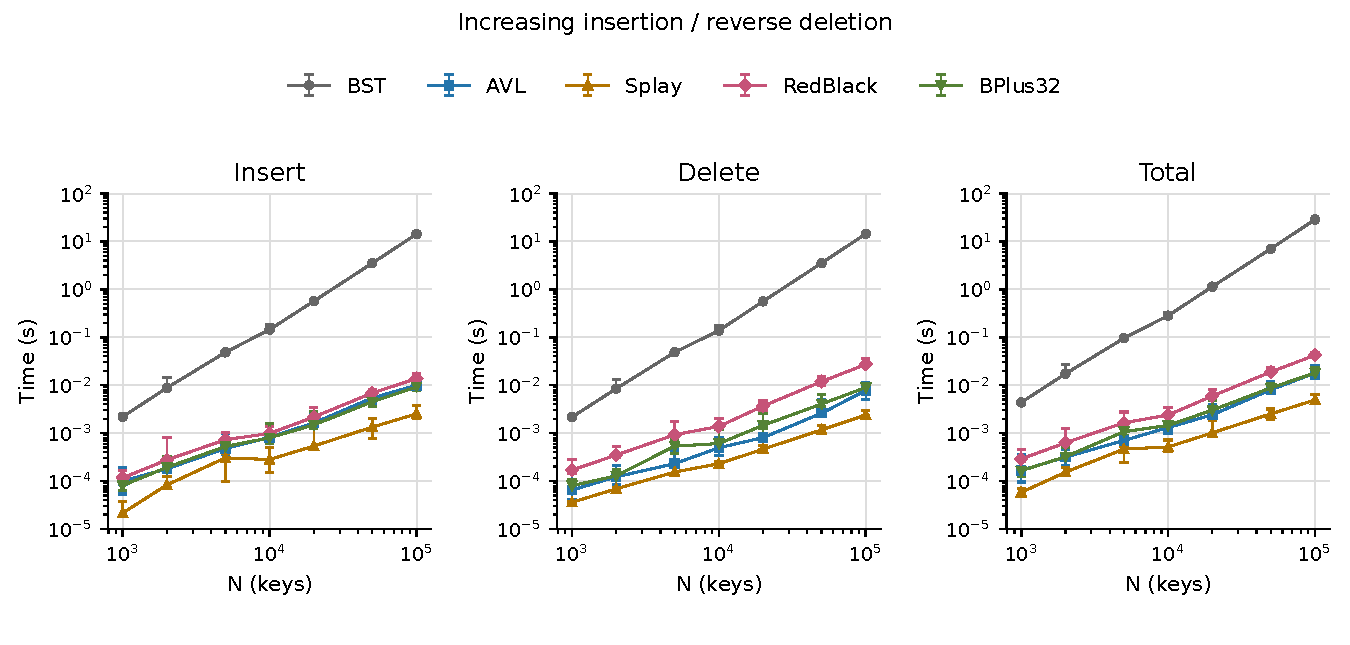
\includegraphics[width=\textwidth]{figures/increasing_reverse.pdf}
\caption{Increasing insertion / reverse deletion. Each phase uses the same scale as its counterpart in the other scenarios.}
\end{figure}

\begin{figure}[htbp]
\centering
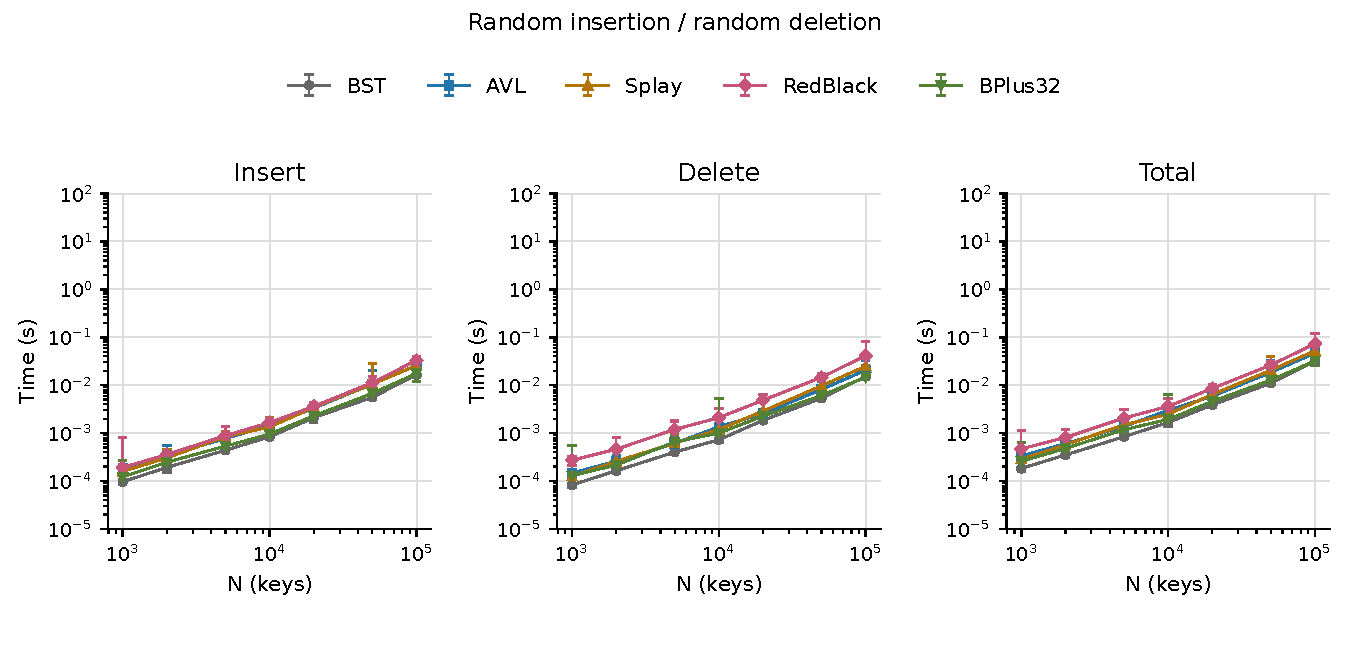
\includegraphics[width=\textwidth]{figures/random_random.pdf}
\caption{Random insertion / random deletion. Each phase uses the same scale as its counterpart in the other scenarios.}
\end{figure}
